
\newcommand\pythonstyle{\lstset{
language=Python,
numbers=left,
stepnumber=1,    
firstnumber=1,
numberfirstline=true
basicstyle=\ttm,
morekeywords={self},              % Add keywords here
keywordstyle=\ttb\color{deepblue},
emph={composite_simpson, composite_trapezoid, func1, mod_composite_simpson, mod_composite_trapezoid, l_i, L, mod1_composite_simpson},          % Custom highlighting
emphstyle=\ttb\color{deepred},    % Custom highlighting style
commentstyle=\color{deepgreen},
frame=tb,                         % Any extra options here
showstringspaces=false
}}


% Python environment
\lstnewenvironment{python}[1][]
{
\pythonstyle
\lstset{#1}
}
{}

% Python for external files
\newcommand\pythonexternal[2][]{{
\pythonstyle
\lstinputlisting[#1]{#2}}}

% Python for inline
\newcommand\pythoninline[1]{{\pythonstyle\lstinline!#1!}}
\subsection{Задание}\label{blockN.VariantM}

\subsubsection*{Условие}
\label{section:условие}
Методы аппроксимации, такие как интерполяция и численное интегрирование, часто используются как составные блоки других, более сложных численных методов. В данной лабораторной работе мы рассмотрим одну из старейших задач вариационного исчисления: задачу о брахистохроне, т.е. задачу о кривой наискорейшего спуска. Она состоит в нахождении такой кривой, по которой материальная точка из точки $(x,y) = (0, 0)$ достигнет точки $(x,y) = (a, y_a)$ под действием силы тяжести за наименьшее время (здесь и далее ось $y$ направлена вниз). Решением этой задачи является такая кривая $y(x)$, которая минимизирует следующий функционал, являющий полным временем движения точки
\begin{equation}
    F = \int\limits_0^a\sqrt{\frac{1+(y'(x))^2}{2gy(x)}dx}, 
\end{equation}
где $g$ обозначает ускорение свободного падения, и $y'(x) = dy/dx$. Эта задача имеет аналитическое решение, которым является параметрически заданная циклоида:
\hypertarget{x}{}
\begin{equation}
    \begin{bmatrix}
    x(t) \\
    y(t)
    \end{bmatrix} = C \begin{bmatrix}
    t - \frac12\sin(2t) \\
    \frac12 - \frac12\cos(2t)
    \end{bmatrix}
\end{equation}
где $t \in [0; T]$ и $C, T$ являются константами, значения которых находятся из граничного условия. В базовой части требуется воспользоваться численным интегрированием для нахождения полного времени движения материальной точки по кривой наискорейшего спуска. В продвинутой части требуется разработать метод для нахождения аппроксимации этой кривой. Здесь и далее принимается $a = 2$ и $y_a = 1$. Константы циклоиды для этого граничного условия равны: $C = 1.0343998$,  $T = = 1.75418438$.
\subsubsection*{Базовая часть}
1. Написать функцию \textit{composite_simpson(a, b, n, f)} численного интегрирования функции $f$ на интервале $[a; b]$ по $n$ узлам с помощью составной формулы Симпсона.\\
2. Написать функцию \textit{composite_trapezoid(a, b, n, f)} численного интегрирования функции $f$ на интервале $[a; b]$ по n узлам с помощью составной формулы трапеций. \\
3. Рассчитать интеграл (\ref{section:условие}) для функции $y(x)$, соответствующей кривой наискорейшего спуска, с помощью составной формулы Симпсона и составной формулы трапеций для множества значений $n \in [3;9999]$. Постройте $log-log$ график зависимости абсолютной погрешности численного интегрирования от шага интегрирования для обеих формул. \\
4. Объясните, каким образом по полученному графику можно определить порядок точности формулы. \\
5. Для обоих формул сравните порядок, полученный с помощью графика, с аналитическим порядком точности. \\
6. Существует ли оптимальный шаг интегрирования для данной формулы, минизимирующий достижимую погрешность? Обоснуйте свой ответ.
\subsubsection{Продвинутая часть}
1. Используя кусочно-линейную интерполяцию с равноудаленными узлами, преобразовать задачу о минимизации функционала (\ref{section:условие}) к полудискретной форме, где аргументами минимизации будут параметры кусочно-линейной интерполяции. \\
2. Далее, используя составную формулу Симпсона, преобразовать задачу к полностью дискретной форме. \\
3. Решить полученную задачу минимизации, используя различные конфигурации дискретизации: с шагом интерполяции и шагом интегрирования от $10^{-3}$ до $1$. \\
4. Используя $log-log$ графики и линии уровня, оценить зависимость погрешности решения от шага интерполяции и шага интегрирования
\subsection{Цель выполнения лабораторной работы}

Цель выполнения лабораторной работы -- \GoalOfResearch.

%----------------------------------------------------------
\subsection{Численное интегрирование}
\subsubsection{1. Составная формула Симпсона}
Необходимо реализовать функцию \textit{composite_simpson(a, b, n, f)} численного интегрирования функции $f$ на интервале $[a; b]$ по $n$ узлам с помощью составной формулы Симпсона. \\
Составная формула Симсона имеет вид: 
\begin{equation*}
    \int\limits_a^bf(x)dx=\frac{h}{3}[f(x_1)+2\sum\limits_{i=1}^{\frac{n}{2}-1}f(x_{2i+1})+4\sum\limits_{i=1}^{\frac{n}{2}}f(x_{2i})+f(x_{n+1})]-\frac{(b-a)h^4}{180}f^(4)(\xi) ,
\end{equation*}
где последнее слагаемое - остаточный член, который при программной реализации численного метода предполагается малым и отбрасывается. \\
\hypertarget{a}{}
\textbf{Программная реализация}:
\begin{python}
def composite_simpson(a, b, n, f):
  k = n - 1 #кол-во промежутков разбиения 
  h = (b-a)/k #шаг разбиения 
  x_nodes = [(a + h*i) for i in range (0,n)]
  sum1 = 2* np.sum([f(x_nodes[2*i]) for i in range (1, int(k/2))]) #сумма значений функции в нечетных узлах 
  sum2 = 4 * np.sum([f(x_nodes[2*i-1]) for i in range (1, int(k/2)+1)]) #сумма значений функции в четных узлах 
  return h/3*(f(x_nodes[0]) + sum1 + sum2 + f(x_nodes[len(x_nodes)-1]))
\end{python}
\subsubsection{2. Составная формула трапеций}
Необходимо реализовать функцию \textit{composite_trapezoid(a, b, n, f)} численного интегрирования функции $f$ на интервале $[a; b]$ по n узлам с помощью составной формулы трапеций. \\
Составная формула трапеций имеет вид: 
\begin{equation*}
    \int\limits_a^bf(x)dx=\frac{h}{2}[f(x_1)+2\sum\limits_{i=2}^{n}f(x_{i})+f(x_{n+1})]-\frac{(b-a)h^2}{12}f''(\xi) ,
\end{equation*}
аналогично п. 1 - остаточный член в программной реализации не учитывается и отбрасывается. \\
\hypertarget{b}{}
\textbf{Программная реализация}:
\begin{python}
def composite_trapezoid(a, b, n, f):
  k = n - 1 #кол-во промежутков разбиения 
  h = (b-a)/k #шаг разбиения 
  x_nodes = [(a + h*i) for i in range (0, n)]
  sum1 = 2* np.sum([f(x_nodes[i]) for i in range (1, n-1)]) #сумма значений функции в нечетных узлах 
  return h/2*(f(x_nodes[0]) + sum1 + f(x_nodes[len(x_nodes)-1]))
\end{python}
\subsubsection{3. Зависимость абсолютной погрешности численного интегрирования от шага интегрирования (формула Симпсона/формула трапеций)}
Необходимо рассчитать интеграл (\ref{section:условие}) для функции $y(x)$, соответствующей кривой наискорейшего спуска, с помощью составной формулы Симпсона и составной формулы трапеций для множества значений $n \in [3;9999]$. Кроме того, необходимо построить $log-log$ график зависимости абсолютной погрешности численного интегрирования от шага интегрирования для обеих формул. \\
Изначально необходимо преобразовать подынтегральную функцию функционала (\ref{section:условие}), используя соотношение (\hyperlink{x}{2}):
\begin{equation}
    dx = \frac12C[2dt - 2\cos(2t)dt] = C[1-\cos(2t)]dt  
\end{equation}
\begin{equation}
    dy = \frac12C[0 - \sin(2t)2dt] = C\sin(2t)dt
\end{equation}
\begin{equation}
    y' = \frac{dy}{dx}=\frac{dy}{dt}\frac{dt}{dx}=
    \frac{Csin(2t)dt}{C[1-\cos(2t)dt}=\frac{\sin(2t)}{1-\cos(2t)}
\end{equation}
Используя (3), (4), (5) преобразуем подынтегральную функцию функционала (\ref{section:условие}):
\begin{equation}
    F = \frac{1}{\sqrt{2g}}\int\limits_0^{t_a}\sqrt{\frac{(1+\frac{\sin(2t)}{1-\cos(2t)})^2}{\frac12C[1-\cos(2t)]}}C[1-\cos(2t)]dt, 
\end{equation}
где $t_a = T$. \\
Подынтегральную функцию функционала будет рассчитывать функция $func1$, которая буквально возвращает значение рассматриваемой функции в некоторой передаваемой точке $t$:
\begin{python}
def func1(t):
  return (1/np.sqrt(2*9.8))*np.sqrt((1+((np.sin(2*t))/(1-np.cos(2*t)))**2)/(1/2 *C * (1-np.cos(2*t))))*C*(1-np.cos(2*t))
\end{python}
Значения вектора $t$ - вектора абсцисс узлов, будут рассчитываться при каждом выборе шага, учитывая, тот факт, что узлы должны быть равномерно-распределенными. 
Кроме, того, необходимо найти точное значение функционала (\ref{section:условие}). Это можно сделать продолжая эквивалентные преобразования соотношения (6), итог которых сведется к следующему:
\begin{equation}
    F = \sqrt{\frac{2C}{g}}\int\limits_0^{t^a}=\sqrt\frac{2C}{g}(T - a),
\end{equation}
где $a = 10^{-7}$, то есть нижняя граница интегрирования должна быть смещена от нулевого значения немногим вправо, т. к. подынтегральное выражение в точке ноль расходится. Этот факт необходимо учитывать и при численном интегрировании, соответственно нижний предел интегрирования соотношения (6) так же равен $a$. \\
\textbf{Программная реализация}:
\begin{python}
a = 10e-7
b = 1.75418438
C = 1.03439984
exact_value_of_integral = np.sqrt(2*C/9.8)* (T - a)
plt.figure(figsize = (10, 7))
plt.loglog()
plt.title("Dependence of the integration error on the step", fontsize = 16)
for i in range (3, 10000, 10):
  k = i - 1
  h = (b-a)/k
  approx_value = mod_composite_simpson(h, i, func1)
  line1 = plt.scatter(h, abs((approx_value - exact_value_of_integral)), s = 17, color = 'violet')


for i in range (3, 10000, 10):
  k = i - 1
  h = (b-a)/k
  approx_value = mod_composite_trapezoid(h, i, func1)
  line2 = plt.scatter(h, abs((approx_value - exact_value_of_integral)), s = 17, color = 'blue')
line1.set_label("Simpson error")
line2.set_label("Trapezoid error")
plt.legend(fontsize = 16)
plt.xlabel('h',fontsize = 16 )
plt.ylabel('error', fontsize = 16)
plt.grid()
plt.show()
\end{python}
Код функций \textit{mod_composite_simpson} и \textit{mod_composite_trapezoid} не приводится для большей лаконичности изложения. Эти функции отличаются от прототипов в п. \hyperlink{a}{1} и п. \hyperlink{b}{2} только принимаемыми аргументами, и это было сделано для субъективного удобства. 
\begin{figure}[h]
\hypertarget{f}{}
\center{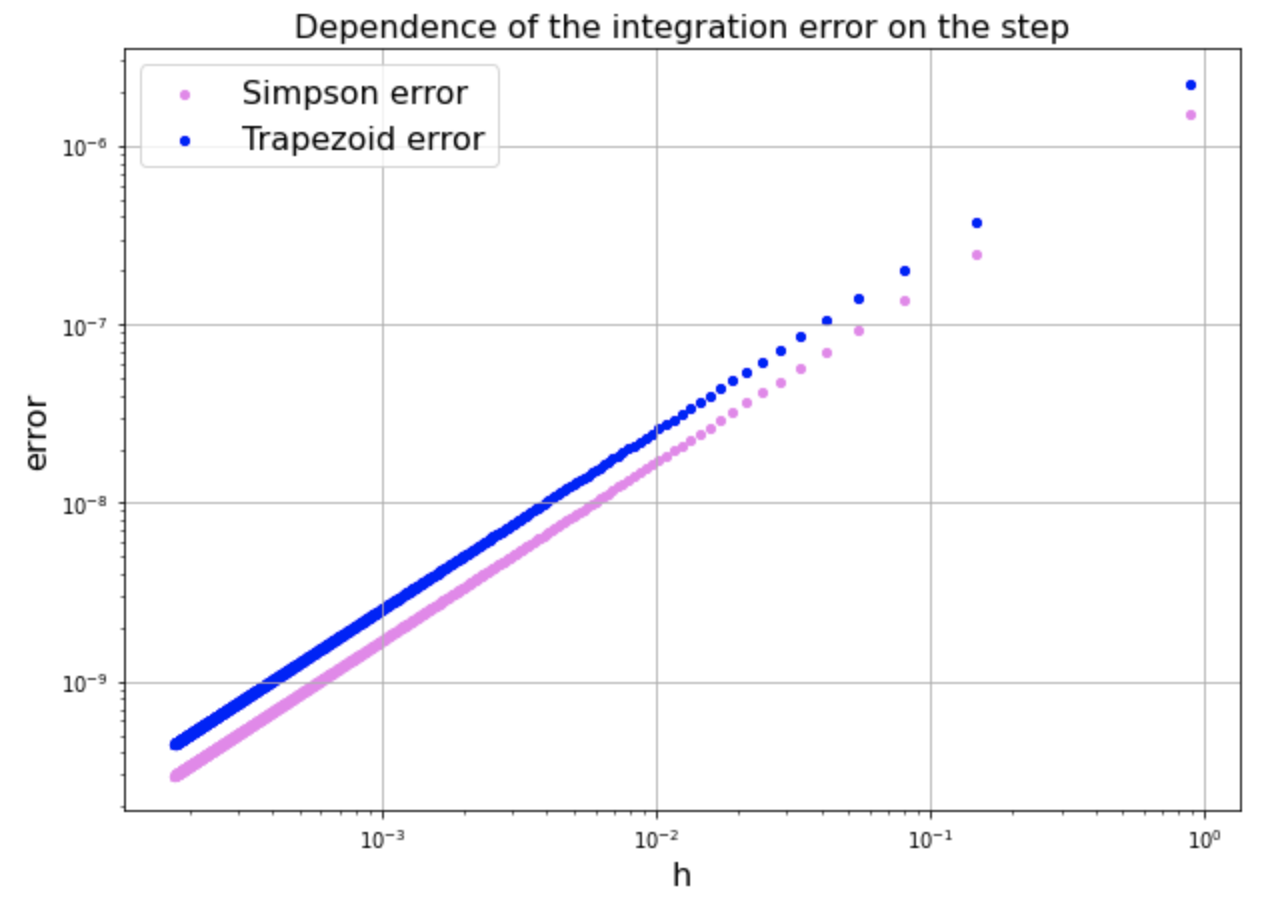
\includegraphics[scale=0.6]{error_steps}}
\caption{Зависимость абсолютной погрешности численного интегрирования от шага интегрирования для составных формул Симпсона и трапеций.}
\end{figure}
\subsubsection{4. Порядок точности}
По полученному графику порядок точности можно определить, например, выведя на одном графике зависимость абсолютной погрешности от шага и аналитическую зависимость формулы от шага. То есть, для достаточно гладких функций, зависимость погрешности от шага, полученная на графике, должна совпадать с аналитической зависимостью. Осуществим это в рамках рассматриваемой задачи, однако, пусть подынтегральной функцией будет достаточно гладкая функция - exp(x).
\begin{figure}[h]
\center{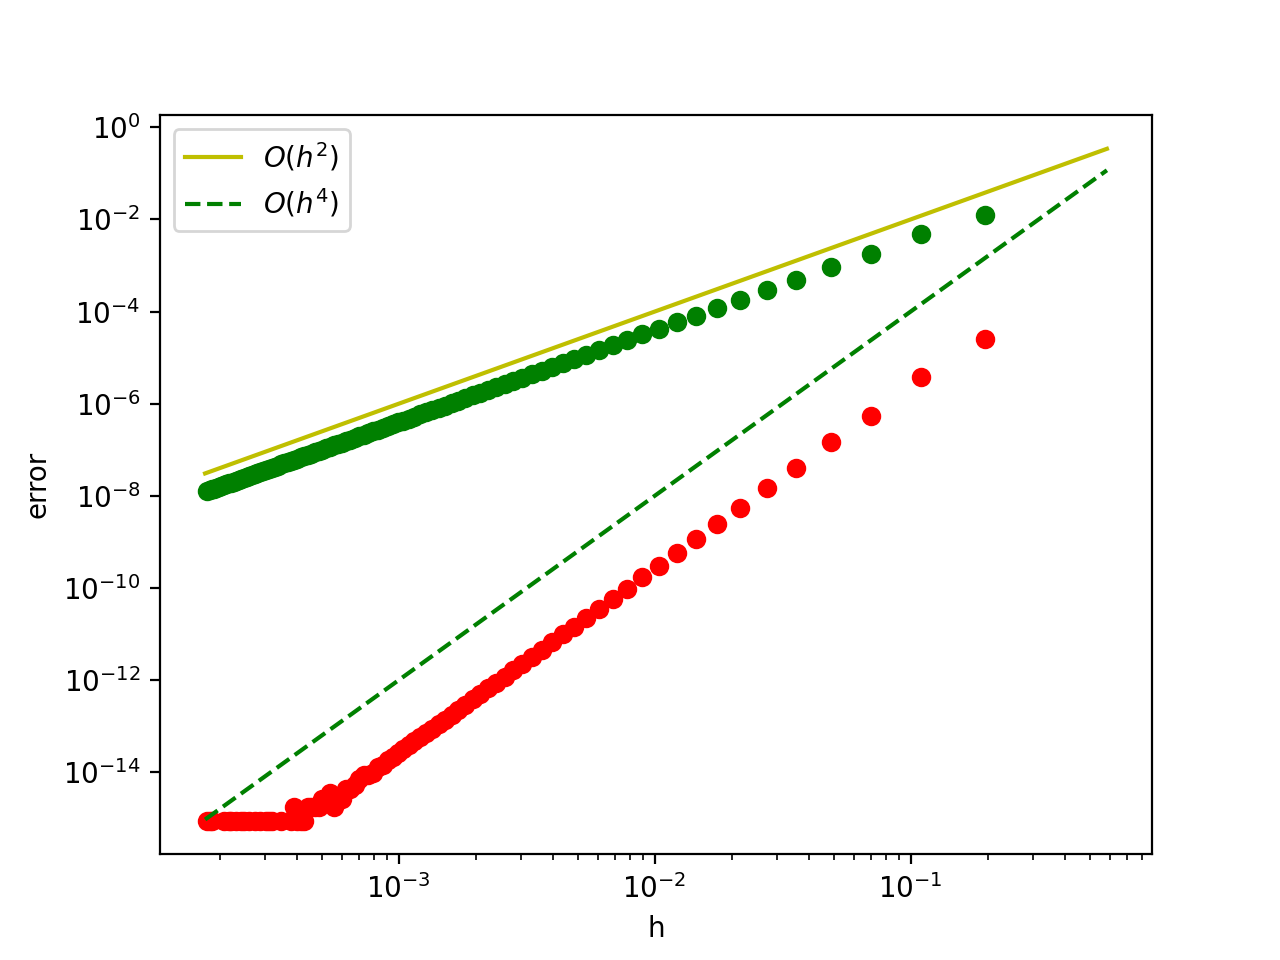
\includegraphics[scale=0.6]{exp}}
\caption{Зависимость абсолютной погрешности численного интегрирования от шага интегрирования для составных формул Симпсона и трапеций. Подынтегральной функцией является достаточно гладкая функция - $\exp(x)$}
\end{figure}
\subsubsection{5. Сравнение порядков точностей для обеих формул (аналитические/полученные из графика)}
Полученные порядки точности из графиков не совпадает с аналитическими порядками точностей ни для формулы Симпсона (4-ый порядок точности), ни для формулы трапеций (2-ой порядок точности). \\
Причин этому несколько:
\begin{enumerate}
	\item  Подыинтегральное выражение в точке ноль расходится.
	\item Расмматриваемая функция (\ref{section:условие}) не является достаточно гладкой.
\end{enumerate}
\subsubsection{6. Оптимальный шаг интегрирования}
Т. к. операция интегрирования является вычислительно устойчивой, то уменьшение шага приводит к более точной аппроксимации и, соответственно, к меньшей погрешности. Что наглядно видно из полученного графика п. \hyperlink{f}{3}.
Следовательно, в реалиях нашей задачи, оптимальным шагом можно считать наименьший рассматриваемый шаг. 
%----------------------------------------------------------
\subsection{Нахождение наилучшей аппроксимации}
\subsubsection{1. Преобразование задачи к полудискретной форме}
Необходимо преобразовать задачу к полудискретной форме, используя кусочно-линейную интерполяцию с равноудаленными узлами. То есть, необходимо построить кусочно-линейный интерполянт для подынтегральной функции. Кол-во линейных интерполянтов (прямых) будет определять кол-во интерполяционных узлов и, соответственно, шаг интерполяции. \\
Для решения данной задачи, модернизируем функции из прошлой лаб. работы: \textit{l_i(i, x, x_nodes)} и  \textit{L(x, x_nodes, y_nodes)}, которые в изначальной реализации считали полином Лагранжа степени $n-1$, где $n$ - кол-во узлов интерполяции. В новой реализации данные функции будут возвращать значение линейных интерполянтов (прямых) в заданной точке. 
\begin{python}
def l_i(x, x_cur, x_ncur):
  k = (x - x_ncur)/(x_cur - x_ncur)
  return (x - x_ncur)/(x_cur - x_ncur)

def L(x, x_nodes, y_nodes):
  for i in range (0, len(x_nodes)-1):
    if (x_nodes[i]<= x <= x_nodes[i+1]):
      return y_nodes[i]*l_i(x, x_nodes[i] , x_nodes[i+1]) + y_nodes[i+1]*l_i(x, x_nodes[i+1], x_nodes[i])

\end{python}
Далее, изобразим на одном графике изначальную функцию и функцию, построенную с помощью линейных интерполянтов для изначальной функции.
\\\textbf{Программная реализация}
\begin{python}
plt.subplots(figsize = (10, 10))
a = 10e-7
b = 1.75418438
t = np.linspace(a, b, 20)
f1 = [func1(t[i]) for i in range (0, len(t))]
t1 = np.linspace(a, b, len(t)*2)
interp_lagr = [L(t1[i], t, f1) for i in range (0, len(t1))]
plt.plot(t1, interp_lagr, label = 'interpolation of lagrange', color = 'green') 
plt.plot(t, func1(t), label = 'real function F[y]', color = 'brown')
plt.legend(fontsize = 16)
plt.xlabel('t',fontsize = 16 )
plt.ylabel('y',fontsize = 16 )
plt.grid()
plt.show()
\end{python}
\begin{figure}[h]
\center{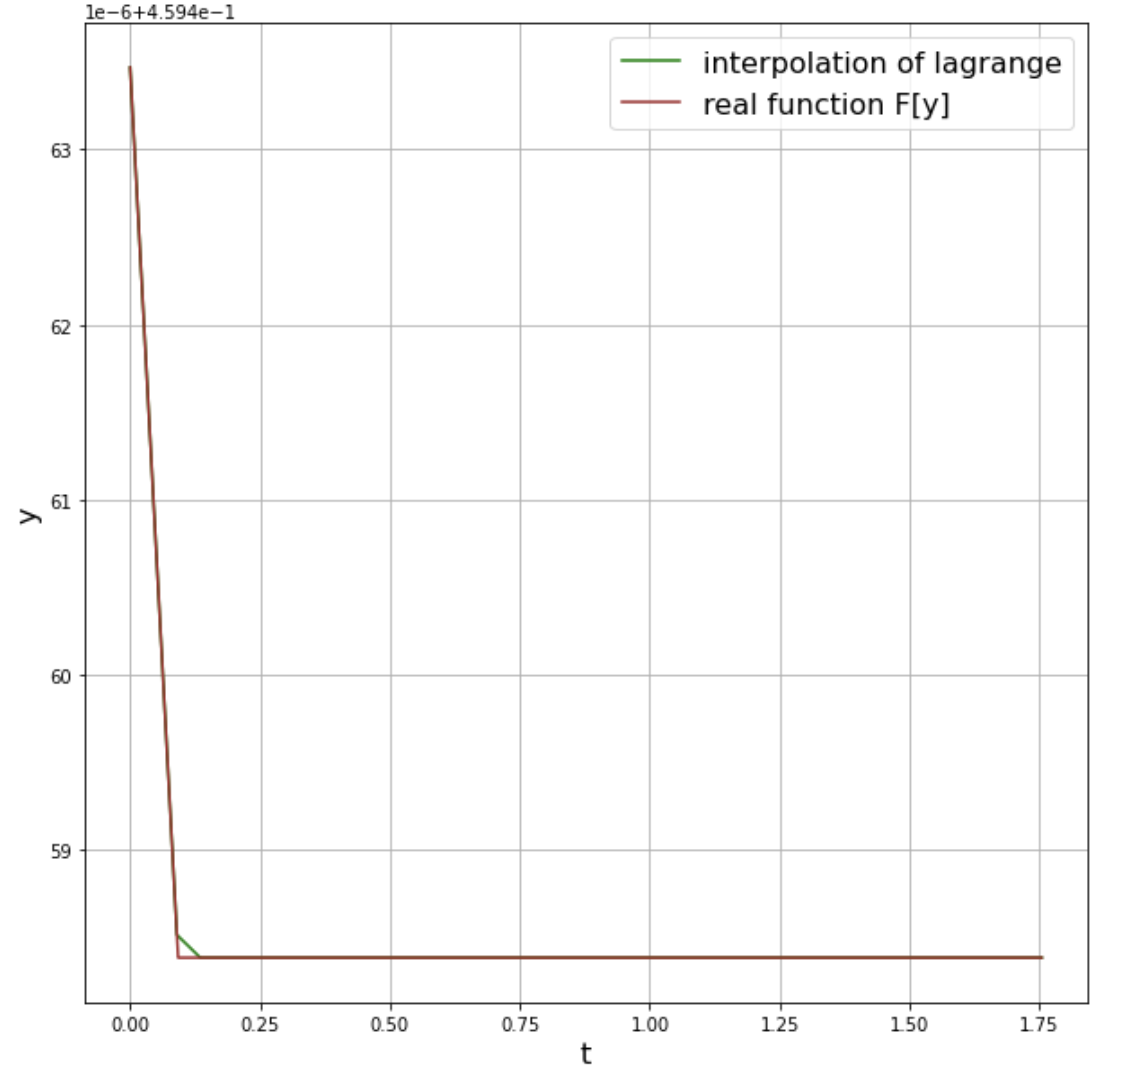
\includegraphics[scale=0.6]{real}}
\caption{График подыинтегральной функции функционала \ref{section:условие} (коричневый) и функции, построенной с помощью линейных интерполянтов (зеленый)}
\end{figure}
\subsubsection{2. Преобразование задачи к полностью дискретной форме}
Необходимо, используя составную формулу Симпсона, привеcти задачу к полностью дискретной форме. То есть, необходимо найти аппроксимацию каждого линейного интерполянта, используя формулу Симпсона. Таким образом, осуществив это, задача сведется к полностью дискретной форме, где аргументами минимизации будут шаг интерполяции и шаг интегрирования. \\
Для реализации этого, вновь модернизируется функция \textit{composite_simpson} - добавляется параметр, являющейся функцией (теперь таких параметров - 2). 
\begin{python}
def mod1_composite_simpson(r, n, f1, L, t):

  sum1 = 0
  sum2 = 0
  for i in range (1, n-1):
    if i % 2 == 0:
      sum1 = sum1 + L(t1[i], t, f1)  #сумма значений функции в нечетных узлах 
    else:
      sum2 = sum2 + L(t1[i], t, f1) #сумма значений функции в четных узлах 
  return r/3*(L(t[0], t, f1) + 2 * sum1 + 4 * sum2 + L(t[len(t)-1], t, f1))
\end{python} 
Здесь функция $L$ - вышеупомянутая функция для подсчета значения линейного интерполянта в точке. \\
В листинге ниже представлена реализация приведения задачи к полностью дискретному виду.
Здесь за шаг интерполяции буквально отвечает параметр $t1$ - который определяет кол-во интерполяционных узлов. Соответственно, чем больше интерполяционных узлов, тем меньше шаг интерполяции. Кроме того, ниже приведен график зависимости погрешности от шага интерполяции (шаг интегрирования фиксирован и равен $10^{-2}$). \\
\textbf{Программная реализация}
\begin{python}
a = 10e-7
b = 1.75418438
T = 1.75418438
C = 1.03439984
approx_value = 0
exact_value_of_integral = np.sqrt(2*C/9.8)* (T - a)
plt.figure(figsize = (10, 7))
plt.loglog()
plt.title("Integration error depending on the interpolation step (fixed integration step = 10e-3)")
r = 10e-3
for i in range (2, 88, 2):
  t = np.linspace(a, b, i)
  t1 = np.linspace(a, b, 2*len(t)+1)
  i = int(len(t1)/len(t))
  h = (b-a)/len(t1)
  n = int((len(t1)/len(t)) + 1)
  k = 0
  for c in range (0, len(t)):
    t_cur = t1[k:k+n]
    k += n-1
    approx_value = approx_value + mod1_composite_simpson(r, i, f1, L, t_cur)
  plt.scatter(h, abs(approx_value - exact_value_of_integral), s = 17, color = 'green')
  approx_value = 0
plt.xlabel('h_interp', fontsize = 16)
plt.ylabel('error',fontsize = 16 )
plt.show()
\end{python}\\
\clearpage
\begin{figure}[t!]
\center{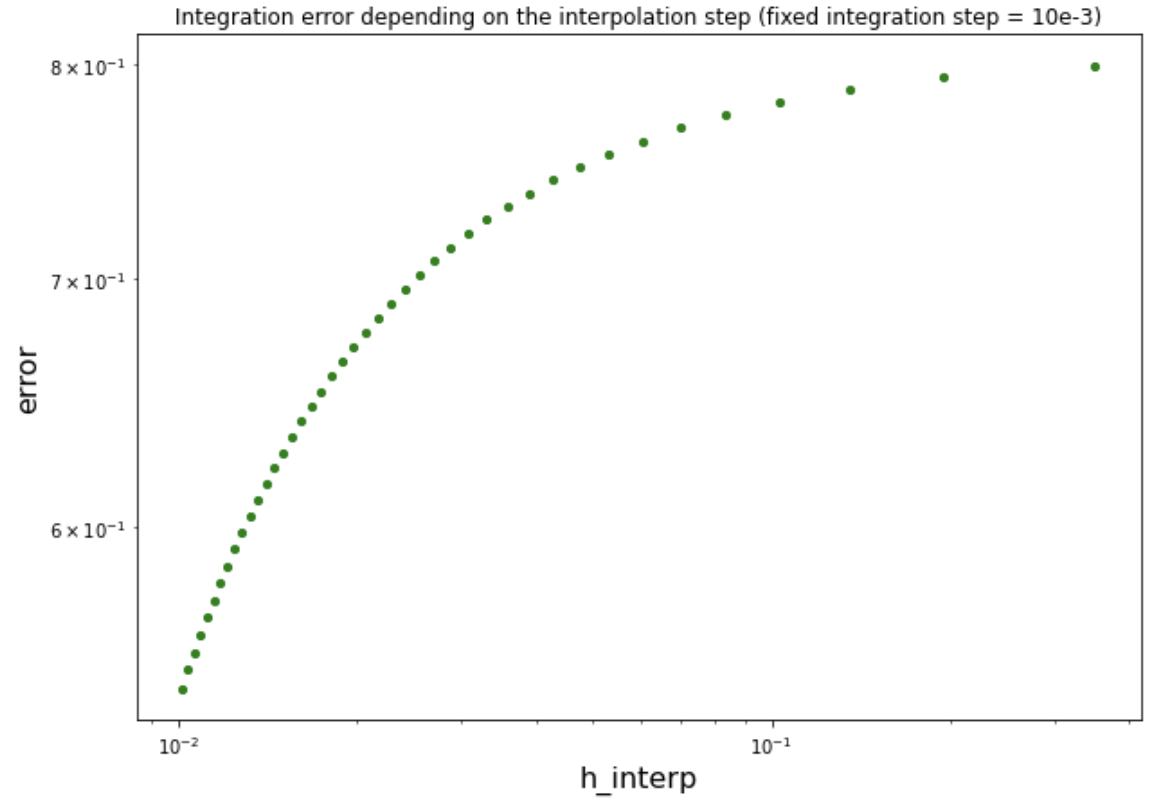
\includegraphics[scale=0.6]{integration_error}}
\caption{Абсолютная погрешность интегрирования в зависимости от шага интерполяции (шаг интегрирования фиксирован и равен $10^{-2}$).\\ Шаг интерполяции варьируется в пределах $[10^{-2}; 1]$}.
\end{figure}
\subsubsection{3. Решение полученной задачи минимизации}
Необходимо решить полученную задачу минимизации (нахождение наилучшего приближения), варьируя параметры минимизации - шаг интерполяции и шаг интегрирования, в пределах $h \in [10^{-3}; 1]$.\\
Как уже ранее было отмечено, операция интегрирования является вычислительно устойчивой, соответственно, меньшая погрешность будет достигаться при меньшем шаге интегрирования. Осуществляя интерполяцию полиномами Лагранжа, можно столкнуться с паразитными осцилляциями, избавиться от которых, вероятно, поможет большее число рассматриваемых линейных интерполянтов и, соответственно, меньший шаг.\\ 
Проверим это: \\
Для этого в листинге кода выше, были добавлены пустые списки \textit{errors} и \textit{steps}, которые будут содержать в себе после очередной итерации текущую погрешность и текущий шаг:
\begin{python}
steps = []
errors = []
steps.append(h)
errors.append(np.abs(approx_value - exact_value_of_integral))
\end{python}
Найдя все погрешности и соответствующие им шаги, найдем минимум погрешности и индекс минимума. По найденному индексу найдем индекс шага.
\begin{python}
val, idx = min((val, idx) for (idx, val) in enumerate(errors))
error_min = val
h_min = steps[idx]
\end{python}
Изобразим на графике зависимость погрешности решения от шага интерполяции. \\Найденный минимум обозначим красным цветом.
\begin{figure}[h]
\center{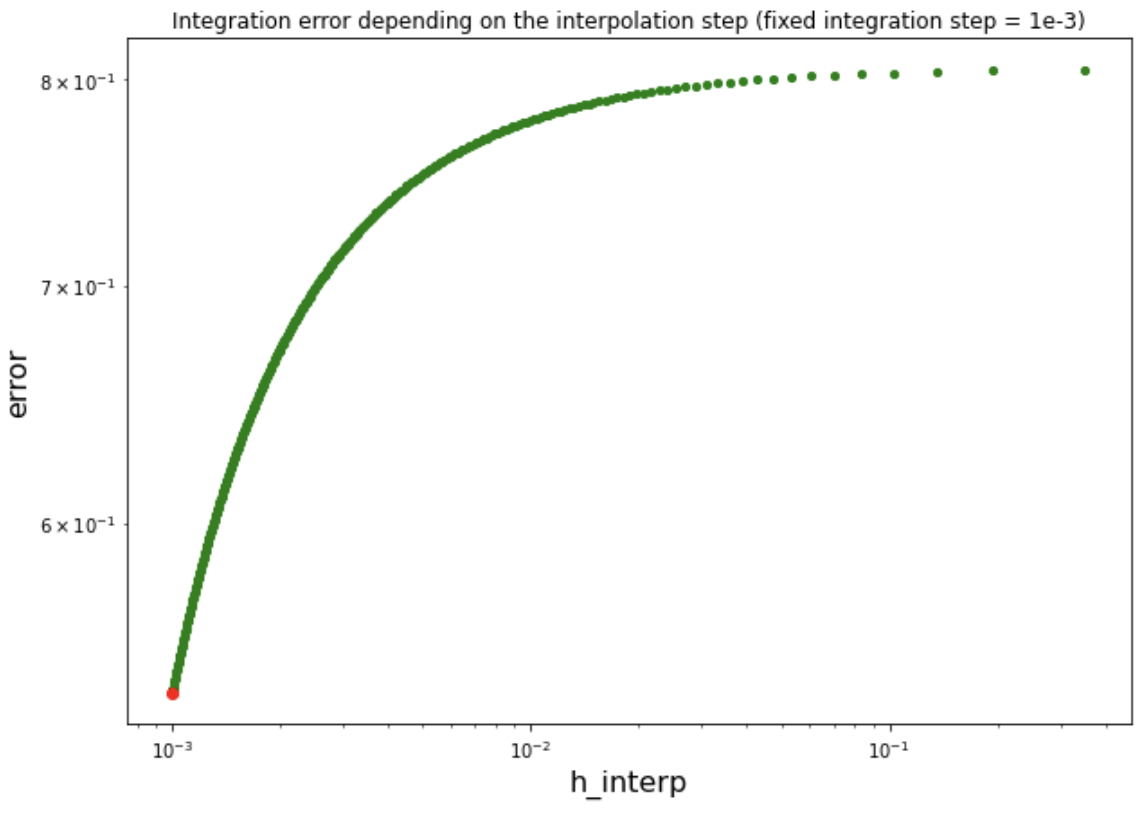
\includegraphics[scale=0.6]{error_red}}
\caption{Абсолютная погрешность интегрирования в зависимости от шага интерполяции (шаг интегрирования фиксирован и равен $10^{-3}$).\\ Шаг интерполяции варьируется в пределах $[10^{-3}; 1].$ Минимум обозначен красным цветом.}
\end{figure}
\subsubsection{4. Оценка погрешности решения в зависимости от шага интегрирования и шага интерполяции}
Необходимо построить $log-log$ график зависимости погрешности от шага интегрирования и шага интерполяции. Шаг интегрирования и шаг интерполяции изменяются в одинаковых пределах $[10^{-3}; 1].$ \\
\textbf{Программная реализация}
\begin{python}
approx_value = 0
exact_value_of_integral = np.sqrt(2*C/9.8)* (T - a)
steps = []
approx_values = []
plt.figure(figsize = (10, 7))
plt.loglog()
plt.title("Integration error depending on the interpolation step and integration step (equal)", fontsize = 14)
r = 10e-3
for i in range (3, 1000, 2):
  t = np.linspace(a, b, i)
  t1 = np.linspace(a, b, 2*len(t)+1)
  i = int(len(t1)/len(t))
  h = (b-a)/len(t1)
  r = h
  n = int((len(t1)/len(t)) + 1)
  k = 0
  for c in range (0, len(t)):
    t_cur = t1[k:k+n]
    k += n-1
    approx_value = approx_value + mod1_composite_simpson(r, i, f1, L, t_cur)
  steps.append(h)
  approx_values.append(np.abs(approx_value - exact_value_of_integral))
  plt.scatter(h, abs(approx_value - exact_value_of_integral), s = 17, color = 'green')
  approx_value = 0
plt.xlabel('h (the interpolation step is equal to the integration step)', fontsize = 12)
plt.ylabel('error',fontsize = 12)
plt.show()
\end{python}
\begin{figure}[h]
\center{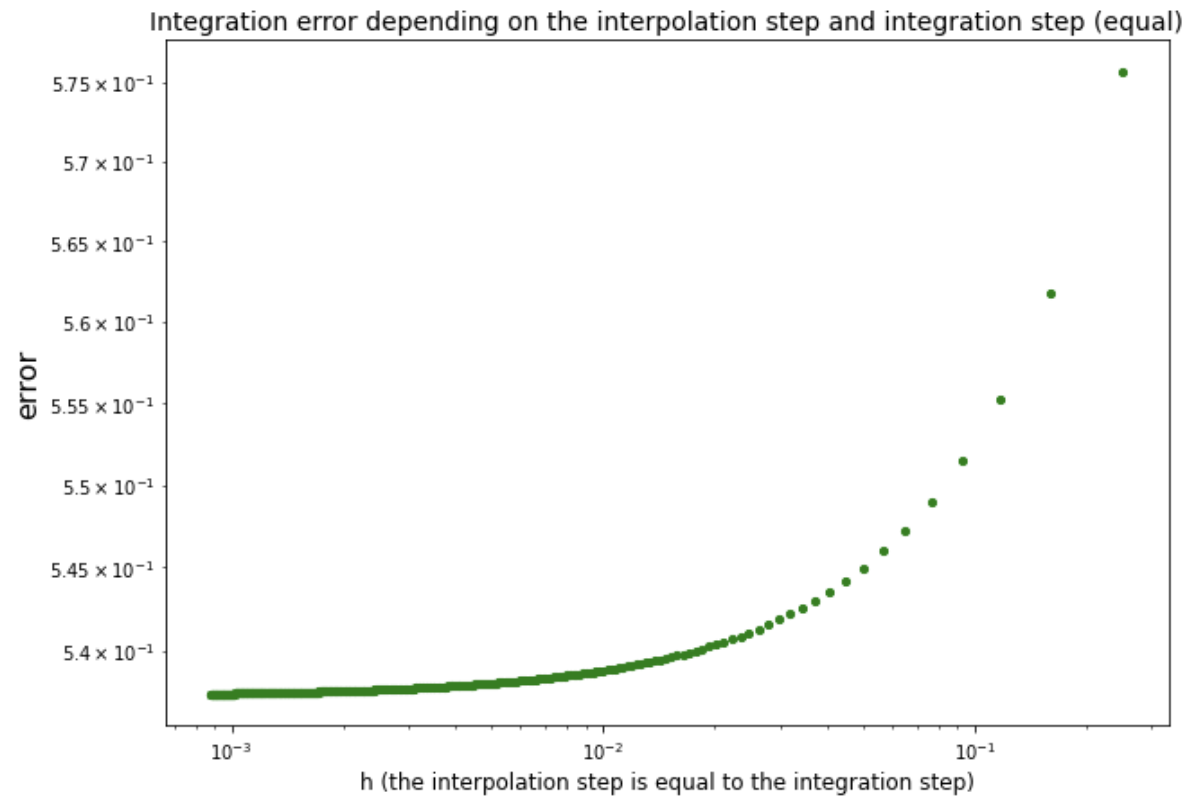
\includegraphics[scale=0.6]{stepsi}}
\caption{Абсолютная погрешность интегрирования в зависимости от шага интерполяции и шага интегрирования (изменяются в равных пределах)}
\end{figure}
\subsection{Заключение}
В ходе данной лабораторной работы было сделано и изучено, а так же проанализировано:
\begin{enumerate}
	\item \textit{Реализация функций численного интегрирования с помощью составной формулы Симпсона и составной формулы трапеций.}
	\item \textit{Нахождение погрешности решения в зависимости от шага интегрирования для обеих формул.}
	\item \textit{Преобразование изначальной задачи к полудискретной форме (посредством линейных интерполянтов Лагранжа).}
	\item \textit{Преобразование полудискретной формы задачи к полностью дискретной форме (с помощью составной формулы Симпсона).}
	\item \textit{Нахождение наилучших шагов интегрирования и интерполяции.}
	\item \textit{Нахождение погрешности решения в зависимости от шага интегрирования и шага интерполяции.}
\end{enumerate}
В совокупности, данная лабораторная работа позволила лучше проработать материал, связанный с понятиями: аппроксимация, численное интегрирование, остаточный член, интерполяция, линейный-интерполянт Лагранжа, абсолютная погрешность.


%----------------------------------------------------------
\subsubsection*{Список использованных источников}

\begin{enumerate}
	\item \bibentry{Pershin2018CompMath}
    \item Першин А. Ю. Видео-лекции по курсу "Вычислительная математика". Москва, 2021
    \textit{https://www.youtube.com/channel/UC69GDhPVLY_7IXn3EhmcH2w}
\end{enumerate}

%----------------------------------------------------------
\subsubsection*{Выходные данные}

\textit{\DocOutReference}
%----------------------------------------------------------
% Атрибуты задачи
\labattributes{}{}{}{}{студент группы \EduGroup, \Author}{\Year, \Semestr}
%----------------------------------------------------------

